\documentclass[11pt]{article}
\usepackage{graphicx}
\addtolength{\oddsidemargin}{-.875in}
	\addtolength{\evensidemargin}{-.875in}
	\addtolength{\textwidth}{1.75in}

	\addtolength{\topmargin}{-.875in}
	\addtolength{\textheight}{1.75in}
	
\usepackage{caption}
\usepackage{hyperref}
\usepackage{color}

\newcommand{\xvec}{\mbox{\bf x}}
\newcommand{\yvec}{\mbox{\bf y}}
\newcommand{\zvec}{\mbox{\bf z}}

\begin{document}

\title{\vspace{-0.25in} Robustness of Nonparametric Regression Using Kernelized Depth Function}
\author{}
\maketitle
\begin{flushleft}

\large

We propose a novel method to reduce the impact of outliers on a given data set using kernelized spatial depth (see Chen et al. (2009)) and the Nadaraya-Watson estimator (see Nadaraya (1964) and Watson (1964)). An `outlier' is an observation that lies at an abnormal distance from other values in a random sample from a population. Generally, outliers are expected to appear more likely in outer layers with small depth values, than in inner layers with large depth values. 

\vspace{0.1in}
\textbf{Spatial Median and Depth}
\vspace{0.1in}

A median is insensitive to outliers as compared to the mean. The multi-dimensional sample median for multi-dimensional data $\{\xvec_1,\ldots,\xvec_n\}$  is any $\xvec \in \mathbf{R}^d$ that satisfies
$$ \parallel \displaystyle{\sum\limits_{i=1}^n S(\xvec_i-\xvec)} \parallel =0,$$
where $\parallel \cdot \parallel$ is the Euclidean distance.
The spatial depth of $\xvec$ for an unknown cdf $F$ is defined as follows (see Vardi and Zhand (2000) and Serfling (2002)):
$$ D(x,\chi) = 1-\frac{1}{\mid \chi \cup \{ \xvec \} \mid-1}  \displaystyle{\parallel \sum\limits_{y \in \chi} S(\yvec-\xvec) \parallel}. $$
Here, $\chi$ is the collection of sample points.
The spatial depth value at median is $1$. 
% The depth attains the maximum value 1 at the deepest point and decreases to zero as a point moves away from the deepest point to the infinity.
Note that this depth function depends only on the sum of unit vectors from point under consideration to the remaining data set.
% Hence it may give a higher depth value for the outliers. 
% To avoid this we use a positive definite kernel  function.\\

\vspace{0.1in}
\textbf{Kernelized Spatial Depth}
\vspace{0.1in}

We now consider a kernelized version of spatial depth as follows:
$$ D_K(\xvec,\chi)= 1-\frac{1}{\mid \chi \cup \{ \xvec \} \mid-1} \left( \displaystyle{ \sum \limits_{\yvec, \zvec \in \chi} \frac{K(\xvec,\xvec)+K(\yvec,\zvec)-K(\xvec,\yvec)-K(\xvec,\zvec)}{\delta_K(\xvec,\yvec) \delta_K(\xvec,\zvec)}}\right)^{1/2},$$ 
where $K(\xvec,\yvec)=exp(-\Vert \xvec-\yvec \Vert^2/\sigma^2)$ and $\delta_K(\xvec,\yvec)=\sqrt{K(\xvec,\xvec)+K(\yvec,\yvec)-2K(\xvec,\yvec)}$. \\ \vspace{0.1in}
Note that $\displaystyle \frac{K(\xvec,\xvec)+K(\yvec,\zvec)-K(\xvec,\yvec)-K(\xvec,\zvec)}{\delta_K(\xvec,\yvec) \delta_K(\xvec,\zvec)}=0$ for $\xvec=\yvec$ or $\xvec=\zvec$.
\vspace{0.1in}

All the above calculations gives us the weight on each of the observation points. If the point lies far away from the data sets, then it has lower weight while if it lies closer to the data sets, then it has higher weight. 
The parameter $\sigma$ determines the size of the neighbourhood that is used to compute KSPD for an observation. When $\sigma$ is 0 then KSPD is constant, and when $\sigma$ is infinity KSPD goes to spatial depth.

\newpage
\vspace{0.1in}
\textbf{Nonparametric Regression}
\vspace{0.1in}

If we have a random sample of bivariate data $(Y_1,X_1),\ldots,(Y_n,X_n)$. The regression model is 
$$Y = m(X) + e,$$ 
where $m$ is an unknown function and $e$ is the random error. Nadaraya and Watson independently proposed the following estimator: 
$$m_{NW}(x)=\frac{\displaystyle{ \sum\limits_{i=1}^n K \left( \frac{X_i-x}{h} \right) Y_i}}{\displaystyle{ \sum\limits_{i=1}^n K \left( \frac{X_i-x}{h}\right )}},$$
where $K(u)=exp(-u^2)$ and $h>0$ is the smoothing parameter.

We modify the Nadaraya-Watson estimator by applying weights to each of the data points as follows:
$$m_{1}(x)= \frac{\displaystyle{ \sum\limits_{i=1}^n D_K(\zvec_i,Z) K\left( \frac{X_i-x}{h} \right) Y_i}}{\displaystyle{ \sum\limits_{i=1}^n D_K(\zvec_i,Z) K\left( \frac{X_i-x}{h}\right )}},$$
where $\zvec_i=(y_i,x_i)$ for $i=1,\ldots,n$ and $Z$ is the collection of $n$ data points. 
This method is well-defined for more feature variables, i.e., multivariate $Y$ as well as multivariate $X$.

\vspace{0.1in}
\textbf{Simulations}
\vspace{0.1in}

{\color{red} Give details here..}

\begin{figure}[ht]
\begin{center}
% \vspace{-0.5in} 
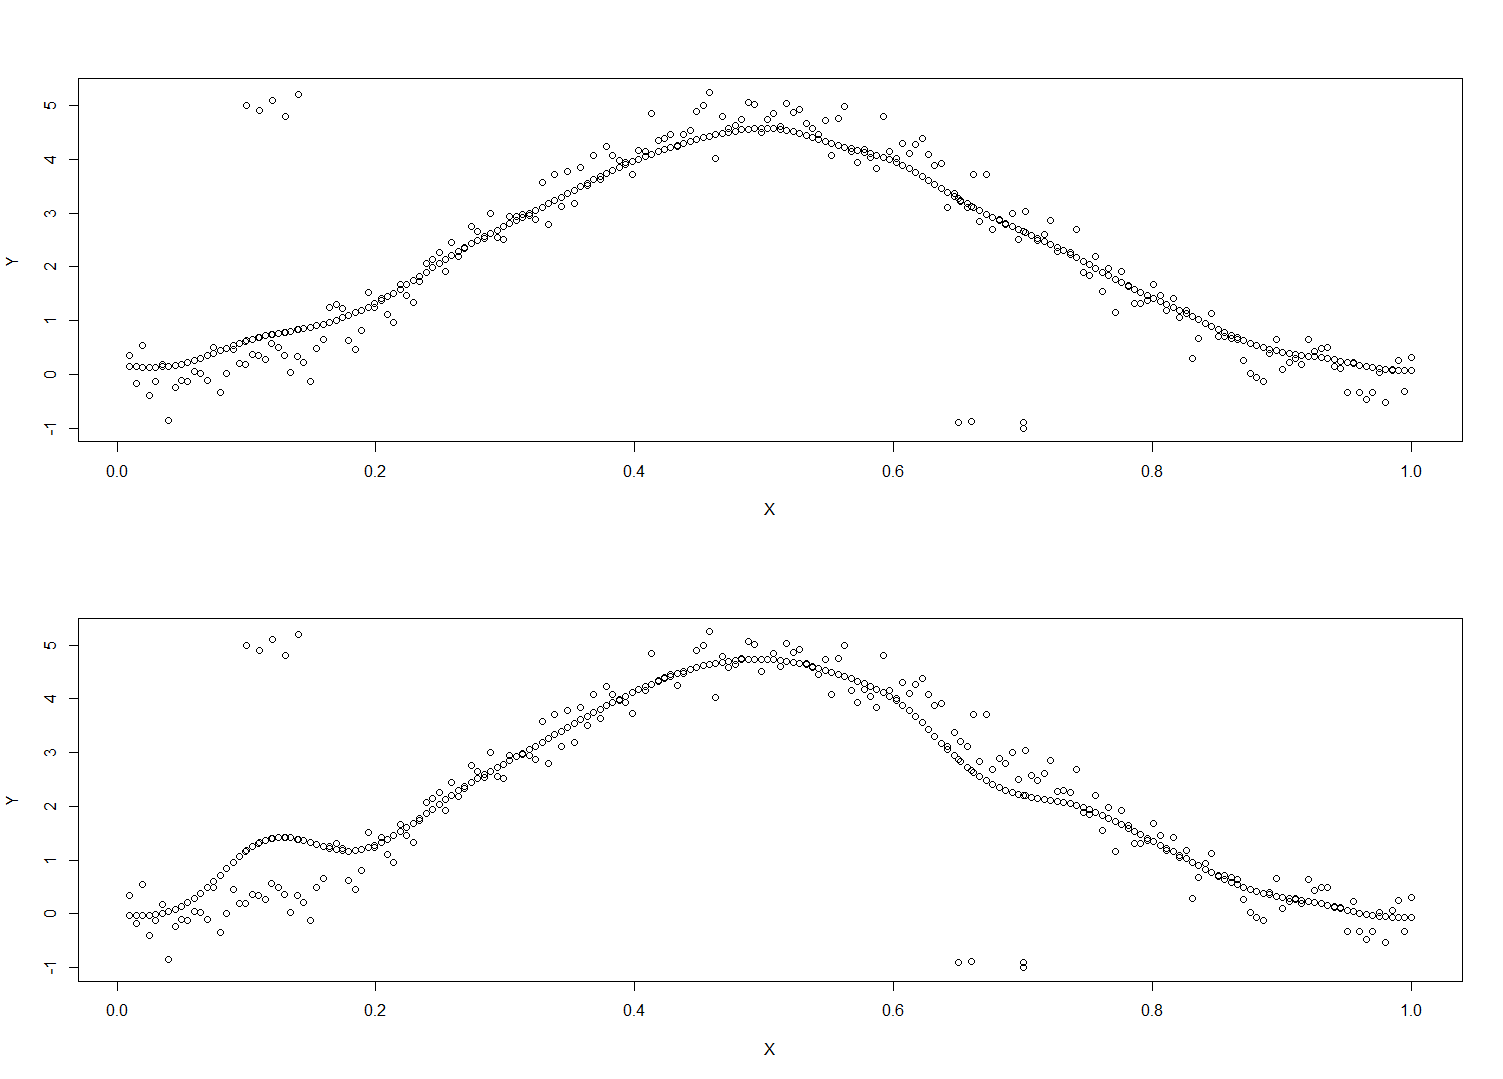
\includegraphics[scale=0.2]{Rplot03}
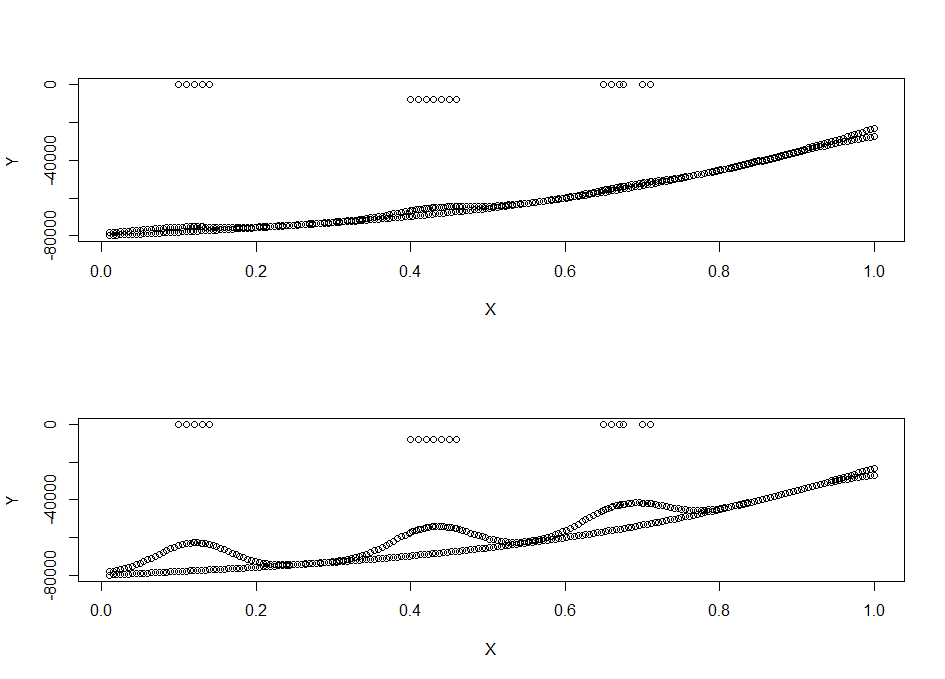
\includegraphics[scale=0.36]{Rplot05}
\end{center}
\end{figure}
 
The lower plot is obtained by the Nadaraya-Watson estimator, and the {\it bulge on the curve} shows the limitation of Nadaraya Watson method on introducing outliers to the data set while the upper plot is obtained by the proposed method.

The simulation was done by varying the parameters $\sigma$ and $h$. We varied $\sigma$ between 0 and infinity to check the impact of the outliers. The smoothing parameter $h$ is obtained by minimizing the error term between the estimated value and the given value. 

\vspace{0.1in}
\textbf{Ongoing Work}
\vspace{0.1in}
\begin{itemize}
 \item We are still working on the part with smoothing parameters.
 \item It will interesting to see how this method works in higher dimensions.
 \item We also want to investigate the performance of the $0-1$ weight function.
\end{itemize}


\vspace{0.2in}
\textbf{References}
\vspace{0.1in}

\small

Chen, Y., Dang, X., Peng, H., and Bart, H. L. (2009) Outlier detection with the kernelized spatial depth function. IEEE Transactions on Pattern Analysis and Machine Intelligence, 31(2), 288-305.
\vspace{0.05in}

% De Brabanter, K., De Brabanter, J., Suykens, J. A., Vandewalle, J., and De Moor, B. (2012) Robustness of kernel based regression: Influence and weight functions. In Neural Networks (IJCNN), The 2012 International Joint Conference on (pp. 1-8). IEEE.
% \vspace{0.05in}

Nadaraya, E. A. (1964) On estimating regression. Theory of Probability and Its Applications, 9(1), 141-142.
\vspace{0.05in}

Serfling, R. (2002) A depth function and a scale curve based on spatial quantiles. In Statistical Data Analysis Based on the L1-Norm and Related Methods (pp. 25-38). Birkhäuser Basel.
\vspace{0.05in}

Vardi, Y., and Zhang, C. H. (2000). The multivariate L1-median and associated data depth. Proceedings of the National Academy of Sciences, 97(4), 1423-1426.
\vspace{0.05in}

Watson, G. S. (1964) Smooth regression analysis. Sankhya: The Indian Journal of Statistics (Series A), 26(4), 359-372.

\end{flushleft}


\end{document}
